\chapter{Technical Approach}
\label{techchap}


https://h2r.cs.brown.edu/writing-a-technical-paper/

Intercalate code

\section{Basic components}

overview of methods. All of the basic components

Mention this because they are important for my work.

Jacobian

Inverse kinematics

Linear system with redundancy

ROS



Wait for this last part

\section{My methods}

My methods. Just implementation in this document.

(Calibration?)

Flacco

QP

\subsection{Kinematic Calibration}

We present a framework for automatic kinematic calibration that leverages an
IMU to accurately estimate the pose (position and orientation) of skin units,
of arbitrary number, along the surface of a robot.

To automatically locate skin units along the surface of a robot,
we utilize the angular velocity and linear acceleration measurements from the IMUs.
Our optimization algorithm estimates the pose (position and orientation) of an SU
using \textit{modified Denavit-Hartenberg (DH) parameters} [1] as illustrated in figure \ref{fig:calibration_theory}.
The pose of each SU is estimated by six DH parameters with respect to the previous
joint in the kinematic chain: four parameters from the joint to a virtual joint,
and two additional parameters from the virtual joint to the SU (other two parameters are set to $0$).
A virtual joint is located within the link that is orthogonal to the joint’s $z$ axis and the SU’s $z$ axis.
This solution is necessary to adhere to the Denavit-Hartenberg notation,
so that each transformation can be expressed with no more than four parameters.

\begin{figure}[htbp]
    \caption[Calibration theory]{
        Depiction of multiple skin units (S) placed on the robots links (L) and separated by joints (J).
        We estimate the Denavit-Hartenberg parameters of each joint in order to calculate the pose of each skin unit along the surface of the robot.
    }
    \begin{center}
    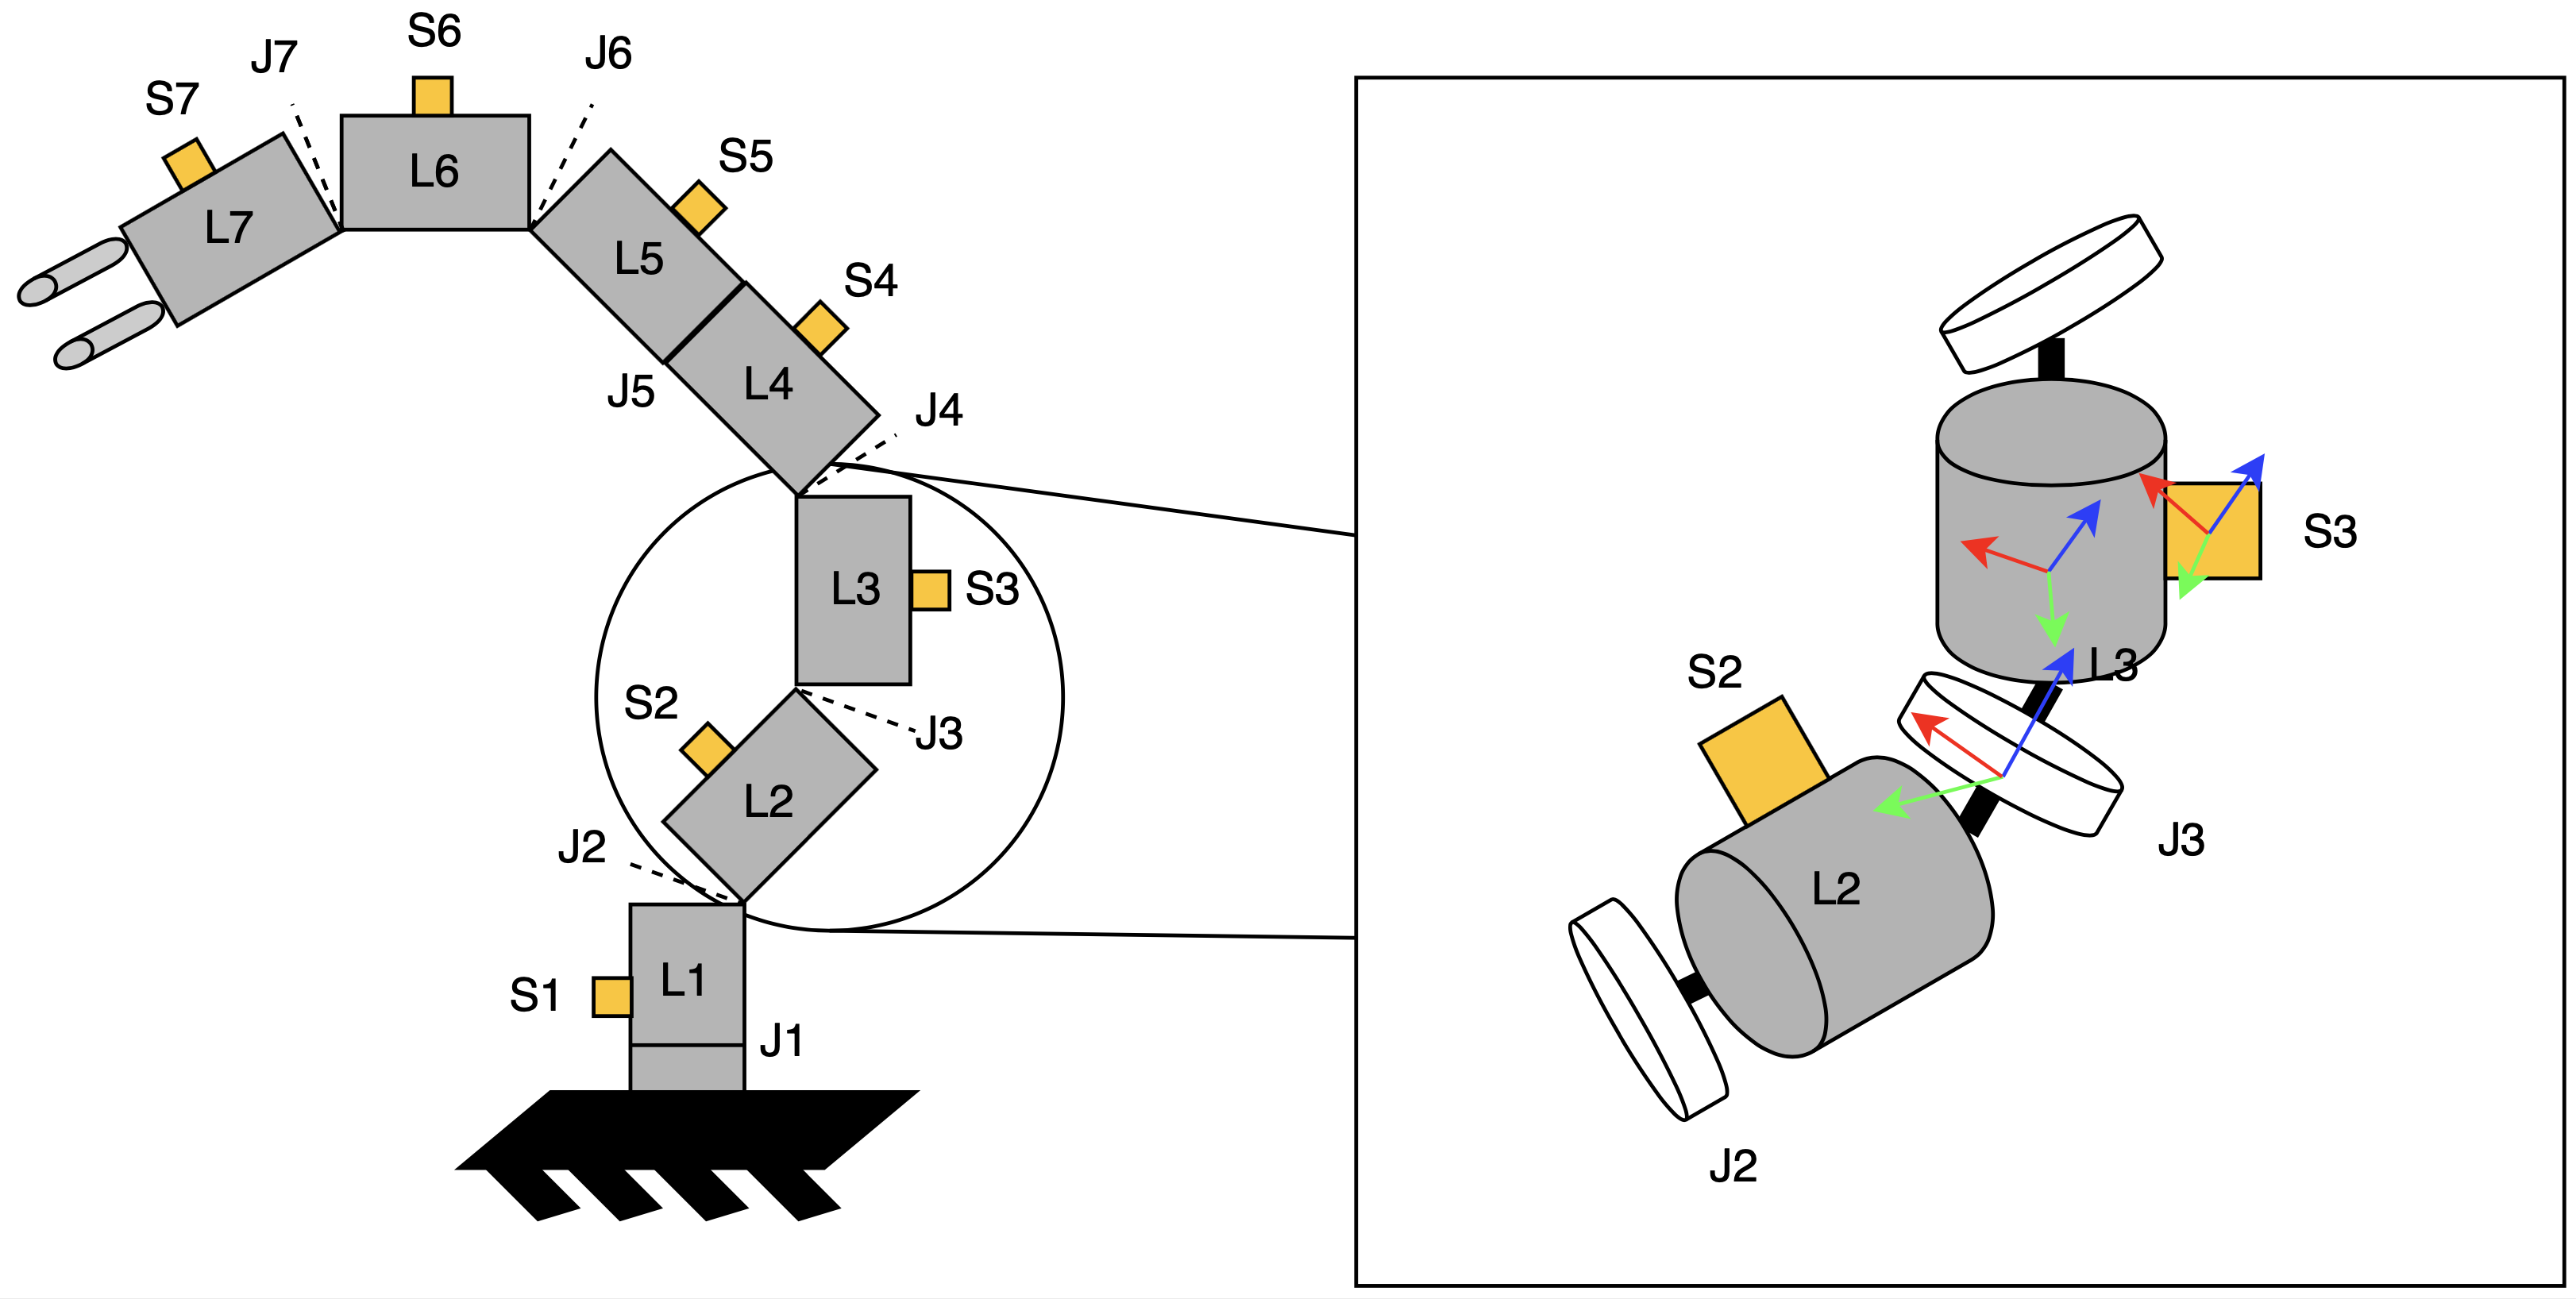
\includegraphics[width=140mm]{figs/calibration_theory.png}
    \end{center}
\label{fig:calibration_theory}
\end{figure}

Our optimization algorithm is composed of the following \textbf{four steps}:

\begin{enumerate}
    \item \paragraph{Initialize a kinematic chain with randomized values.}
    We represent each skin unit coordinate using a transformation matrix.
    $${}^0T_{SU_i} = {}^0T_1 \cdot {}^1T_2 \dots {}^{i-1}T_i \cdot {}^i T_{SU_i}, \quad \forall i$$
    , where:
    $$
    {}^{i}T_{i+1} =
        \left[ \begin{array}{c|c}
            {}^{i}R_{i+1} & {}^{i}P_{i+1} \\
            \hline
            \mathbf{0} & \mathbf{1} \\
        \end{array}\right].
    $$

    \item \paragraph{Collect Data.}
    First, static forces applied to the IMU (that is, the constant acceleration due to gravity)
    are measured and compensated for.
    Then, each reference joint is moved through its operational range in a constant rotation pattern
    and the resulting acceleration as measured by the IMU is stored.

    \item \paragraph{Define an error function.}
    Acceleration exerted on each SU ${}^{SU_i}a_{u,d}$ can be estimated as a composition of local acceleration,
    tangential acceleration and centripetal acceleration:
    $$^{RS}\vec{a}_{t a n_{u, d}} = ^{R S} \overrightarrow{\alpha_{d}} \times^{R S} \vec{r}_{u, d}$$

    $$^{RS}\vec{a}_{cp_{u, d}} = ^{R S} \vec{\omega}_{d} \times\left(^{R S} \vec{\omega}_{d} \times^{R S} \vec{r}_{u, d}\right)$$

    $$^{SU_{i}}\vec{a}_{u, d} = ^{SU_{i}}\underline{R}_{R S} \cdot\left(^{R S} \vec{g}+^{R S} \vec{a}_{t a n_{u}, d}+^{R S} \vec{a}_{c p_{u, d}}\right).$$
    Angular velocity $\omega$ and angular acceleration $\alpha$ are measured during data collection, whereas rotation matrix $R$ and position vector $P$ can be computed using the current estimated DH parameters.

    One example error function could be seen as the error between the measured accelerations from the IMUs and the estimated accelerations using the kinematic chain model for $n_{pose}$ poses [2]:
    $$E = \sum_{i=1}^{n_{pose}} \sum_{j=1}^{n_{joint}} ||a^{model}_{i,j} - a^{IMU}_{i,j}||^2$$

    \item \paragraph{Minimize the error function with a global optimizer.}
    A global optimizer optimizes the DH parameters by minimizing the chosen error function. We combine several different error functions to estimate both rotational and translational parameters. The final result in simulation can be seen in figure \ref{fig:calibration_result}.

\end{enumerate}

\begin{figure}[htbp]
    \caption[Calibration result]{
    Calibrated IMU positions on a simulated Franka Emika Panda robot.
    }
    \begin{center}
    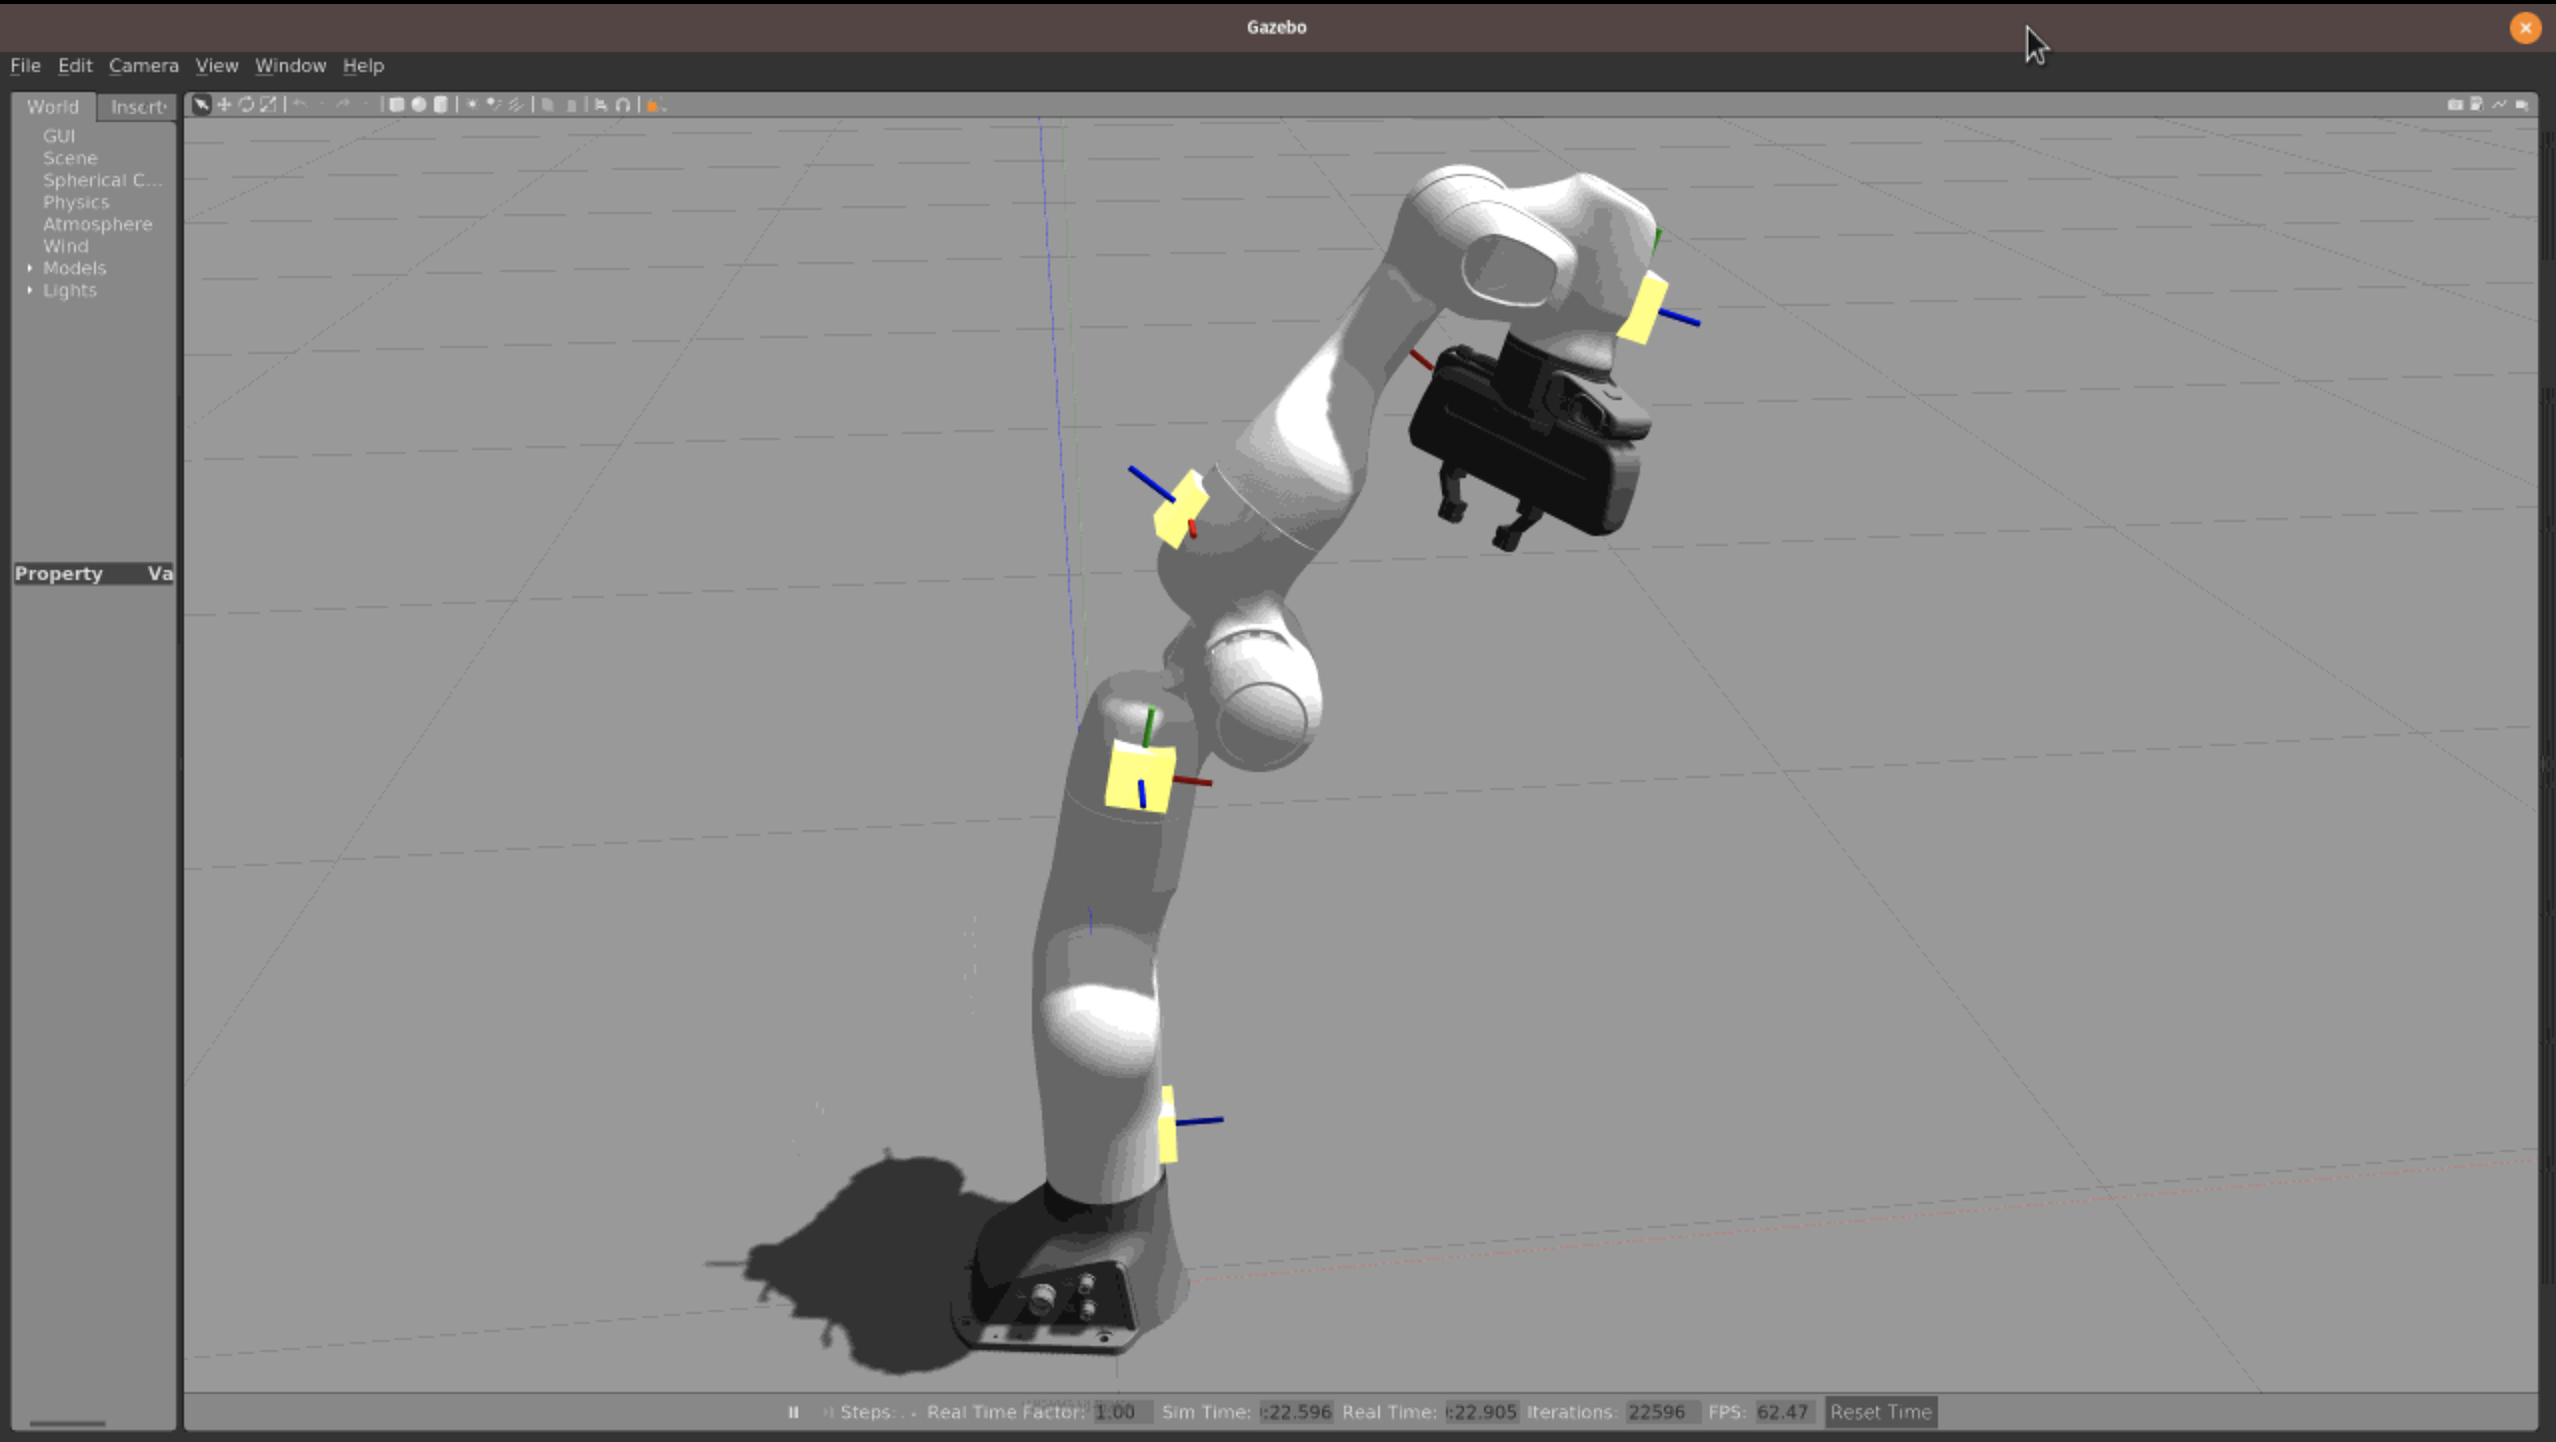
\includegraphics[width=140mm]{figs/calibration_result.png}
    \end{center}
\label{fig:calibration_result}
\end{figure}
